% Saving data, determining equilibirum and correlation

% In practice chose to write the entire length profile to disk to be able to later decide on specific observable, the disk space is still minimal
% In the end we wish to look at the behaviour of the autocorrelation of the length profile for large N, but we have not yet done so
% For simiplicity we have as of yet only look at the behaviour of the std
% We wish to obtain the behaviour of std for large N, for this we wish to use batching to be able to make good estimates of the error
% For this we need estimates of the equilibrium time, to make sure the system is thermalized; and estimates of the correlation time to reduce the amount of data that needs to be saved and to know how big to take the batches

\begin{frame}
    \frametitle{Analysing observables}

    \begin{itemize}
        \item Wanted: \emph{autocorrelation} for $N \rightarrow \infty$ \\[3mm]
        \item As of now: behaviour of \emph{standard deviation}
        \item Batching for error estimates
        \item Required: $t_{eq}$ and $t_{cor}$
    \end{itemize}
\end{frame}

% It is difficult to construct another initial state so we , so to estimate the equilibrium time we use ...
% And we notice the equilibirum time is rather small and constant for different N (in terms of sweeps), because our initial state is very close to equilibirum.
\begin{frame}
    \frametitle{Thermalisation}

    \begin{itemize}
        \item Estimate $t_{eq}$ by convergence \\[3mm]
        \item Equilibrium time is small and size independent % That is in terms of sweeps
        % This can be understood since the generic geometry is not much wilder than the flat geometry.
    \end{itemize}
    \begin{figure}[b]
        \centering
        \begin{minipage}{0.49\linewidth}
            \centering
            % Insert image of convergence of t_eq
            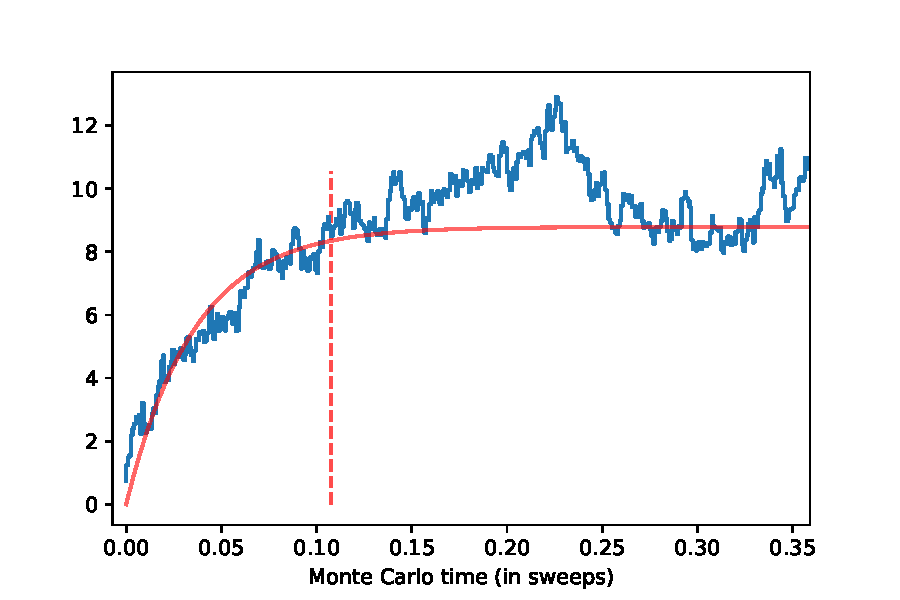
\includegraphics[width=\linewidth]{teq-convergence.pdf}
        \end{minipage}
        \hfill
        \begin{minipage}{0.49\linewidth}
            \centering
            % Insert image of t_eq for different N
            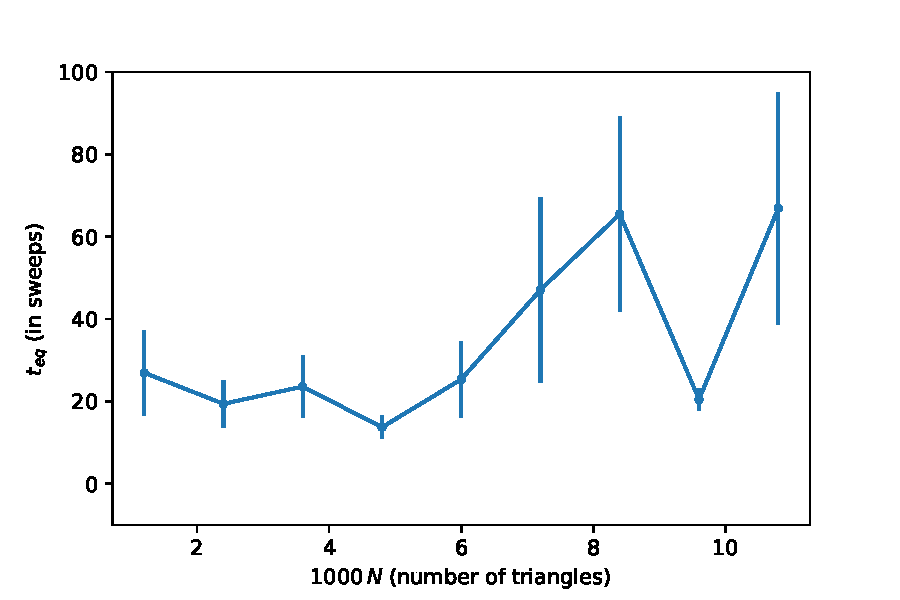
\includegraphics[width=\linewidth]{teq-plot.pdf}
        \end{minipage}
    \end{figure}
\end{frame}

% We have a single model parameter which can still be tuned, so we can tune it to make the correlation time minimal.
% We determine the correlation time be simulation long traces of the std and looking for 'exponential decay' behaviour in the autocorrelation of the std with respect to the simulation step time.
% Determining this for different ratios we see there is a large minimum around 0.4, and notice the correlation time is not very sensitive around this minimum; so it should be save to choose 0.4
\begin{frame}
    \frametitle{Correlations}
    \begin{itemize}
        \item We have the \emph{move ratio} as model parameter
        \item Tune to minimize correlation time
        \item Correlation time is estimated by exponential decay
        \item Choose \emph{move ratio} $0.4$
    \end{itemize}
    \begin{figure}[b]
        \centering
        \begin{minipage}{0.49\linewidth}
            \centering
            % TODO: insert image of exponential decay
            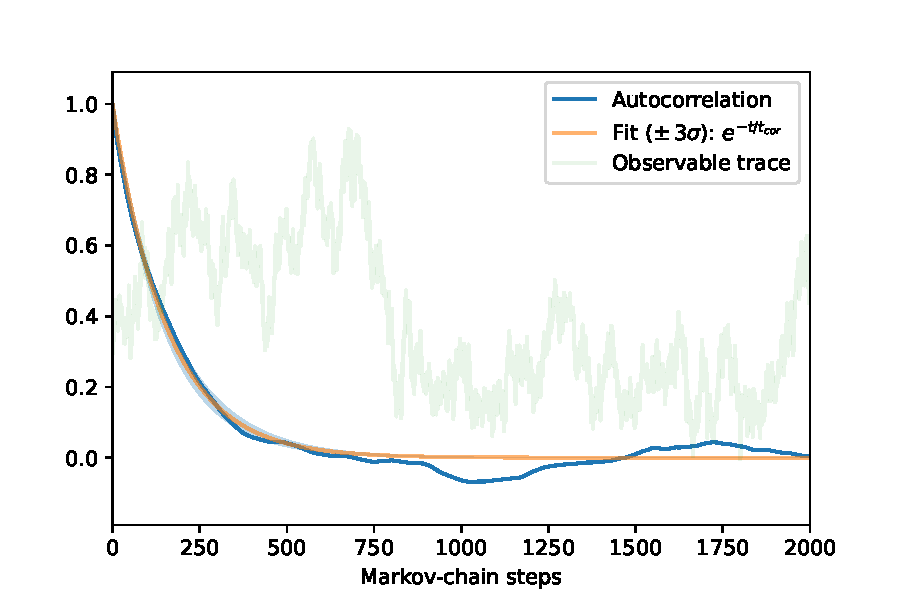
\includegraphics[width=0.95\linewidth]{tcor-decay.pdf}
        \end{minipage}
        \hfill
        \begin{minipage}{0.49\linewidth}
            \centering
            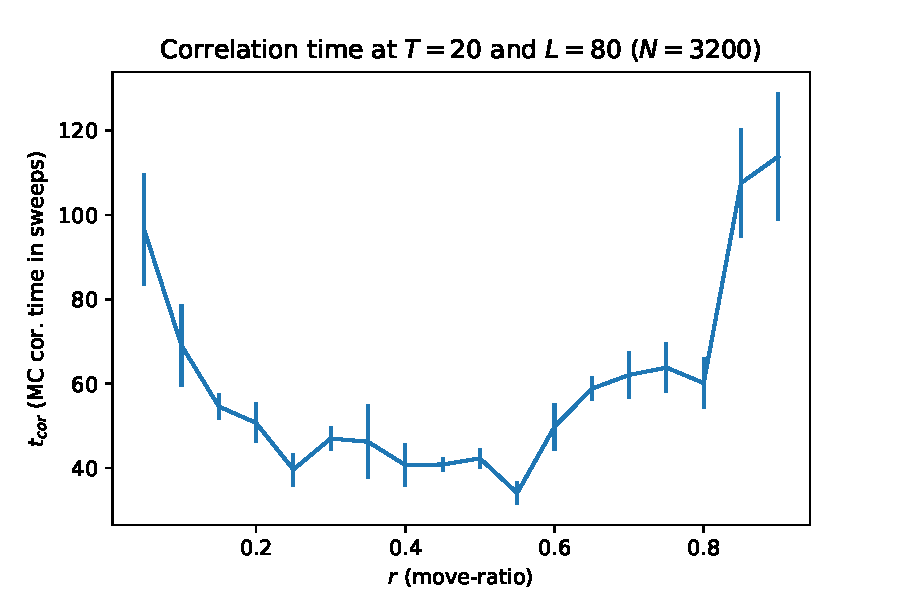
\includegraphics[width=0.95\linewidth]{tcor_r_t20_l80.pdf}
        \end{minipage}
    \end{figure}   
\end{frame}

% We perform similar measurements for different L values, which shows the correlation time is roughly constant; and we look for different T values which suggests tcor grows roughly with O(T).
% Thus in total we find that tcor grows with O(N) in sweeps thus O(N^2) in MC steps, which is very unfortunate as this inhibits us from performing large simulations. But what we can do is keep T constant and make N large
\begin{frame}
    \frametitle{Correlations}
    \begin{itemize}
        \item Find $T$ and $L$ dependence of $t_{cor}$
        \item Constant in $L$
        \item Roughly $\order{T}$ 
        \item So $t_{cor} = \order{N}$ (in sweeps)
    \end{itemize}
    \begin{figure}
        \centering
        \begin{minipage}{0.49\linewidth}
            \centering
            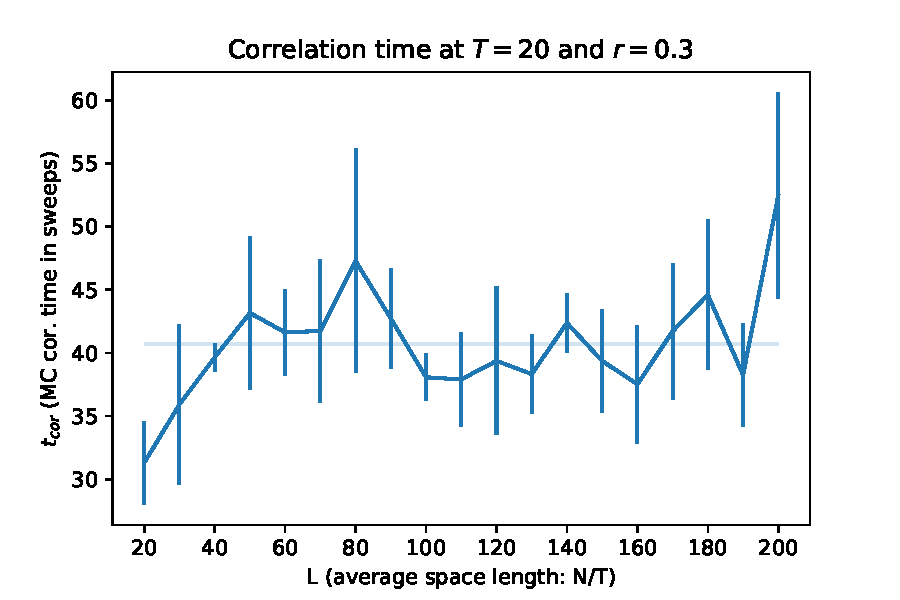
\includegraphics[width=\linewidth]{tcor_l_t20_r0.3.pdf}
        \end{minipage}
        \hfill
        \begin{minipage}{0.49\linewidth}
            \centering
            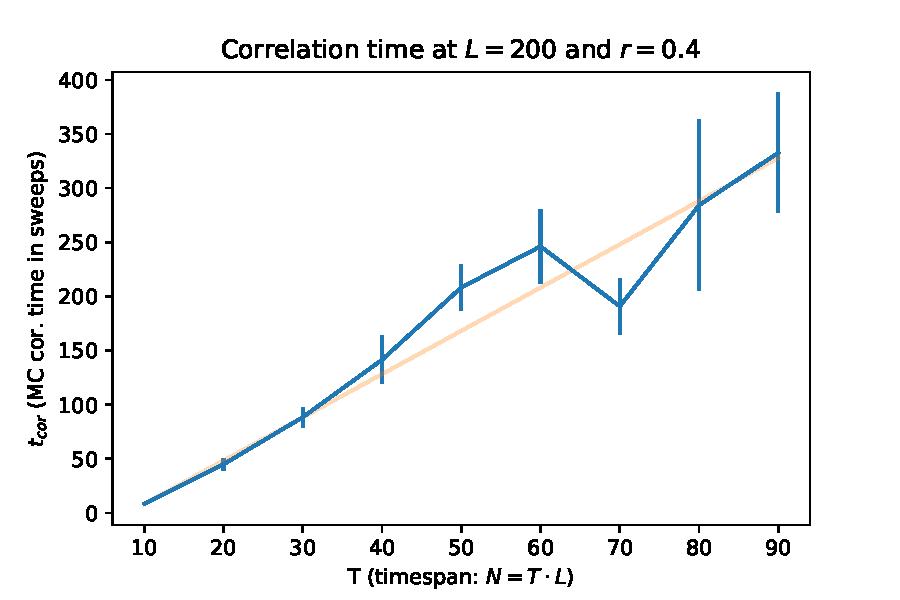
\includegraphics[width=\linewidth]{tcor_t_l200_r0.4.pdf}
        \end{minipage}
    \end{figure}
\end{frame}


\begin{frame}
    \frametitle{Results}
    Variance behaviour: $\sigma(\rho_L) \propto N^{0.50 \pm 0.01}$
    \begin{figure}[b]
        \centering
        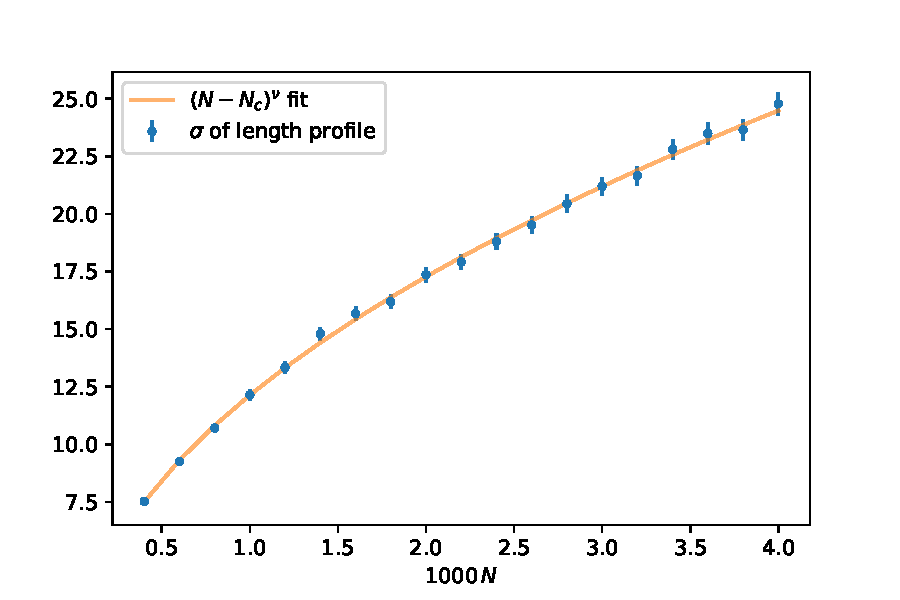
\includegraphics[width=0.8\linewidth]{std-profile.pdf}
    \end{figure}
    % Todo include figure of sigma
\end{frame}
% First results show that std gros as a non-trivial power in N